Esta librería es la encargada de realizar el parsing del documento NCL. Es una de las primeras tareas que se realiza al iniciar Ginga.
Tiene como responsabilidad leer y analizar el documento NCL, detectando posibles errores sintácticos que no estén acorde a lo que especifica la norma.
A medida que se realiza el parsing se van instanciando las clases de \emph{ncl30} correspondientes y se van aplicando las propiedades leídas del documento NCL.
Para realizar el parsing se trata al documento como un archivo XML.\\
Se comienza leyendo el \texttt{head} del archivo buscando por alguno de los elementos clave:
\begin{itemize}[noitemsep,nolistsep]
\item importedDocumentBase.
\item regionBase.
\item ruleBase.
\item transitionBase.
\item descriptorBase.
\item connectorBase.
\item meta.
\item metadata.
\end{itemize}

Y luego, a su vez dentro de cada uno de ellos, los elementos correspondientes a cada sección.
Una vez terminado el parseo del \texttt{head}, se procede a analizar el \texttt{body} buscando las siguientes secciones:
\begin{itemize}[noitemsep,nolistsep]
\item media.
\item context.
\item switch.
\end{itemize}

Cuando se termina de realizar el parsing se retorna un valor indicando si se produjo algún error.

\begin{figure}[h!]
	\centering
	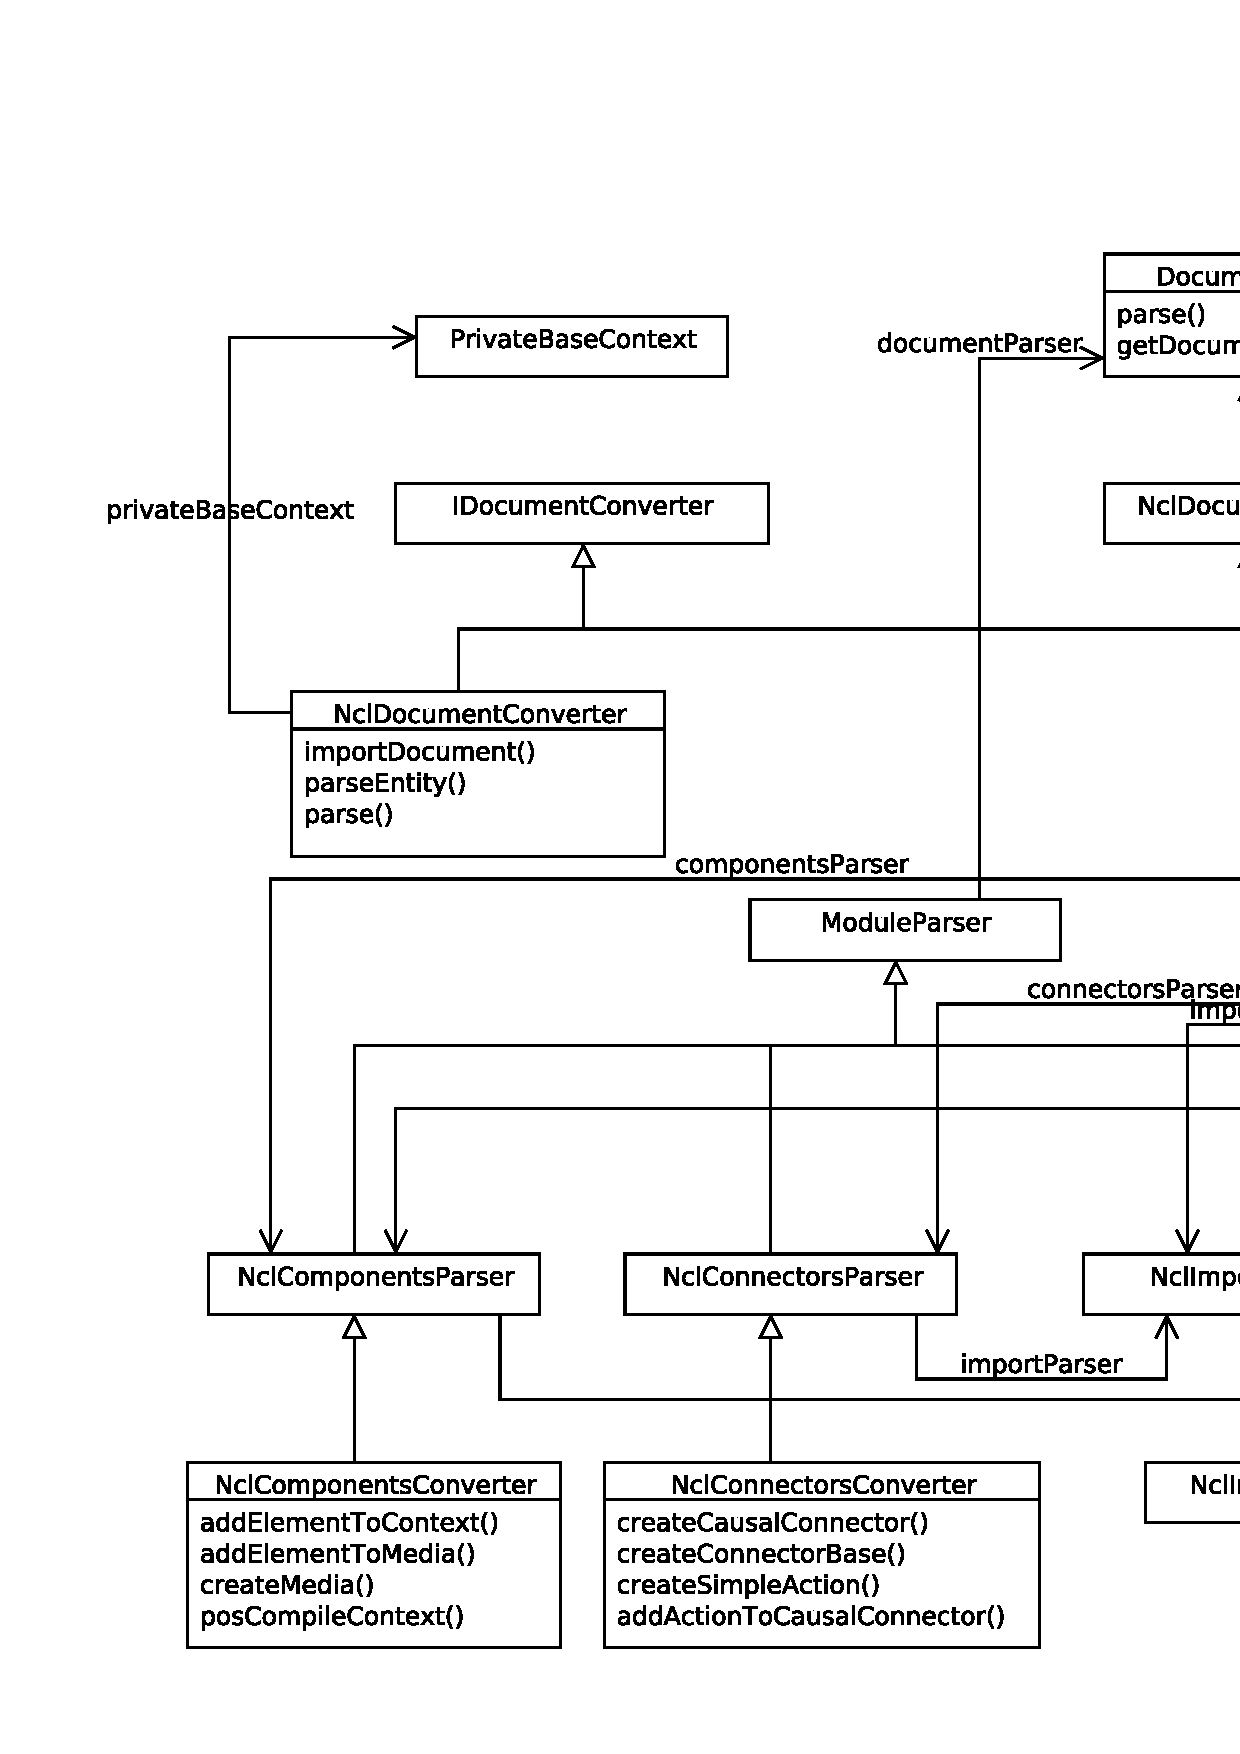
\includegraphics[scale=0.3]{resources/uml-ncl30-converter.jpg}
	\caption{Diagrama de las principales clases de la librería \emph{ncl30-converter}.}
\end{figure}

\FloatBarrier
